\noindent {\bf Chapter editors:}~Giovanna Cottin, Zhen Liu, Andre Lessa, Sabine Kraml\\
\text{ \; }\\
\noindent {\bf WG conveners:}~Juliette Alimena, Will Buttinger, Jared Evans\\
\text{ \; }\\
\noindent {\bf Contributors:}~Eric Conte, Yanou Cui, Nishita Desai, Benjamin Fuks, Jan Heisig, Gavin Hesketh, Lukas Heinrich,  David Michael Morse, Michael Ramsey-Musolf, Ennio Salvioni, Michele Selvaggi, Brian Shuve, Yuhsin Tsai
\text{ \; }\\

%%%%%%%%%%%%%%%%%%%%%%%%%%%%%%%%%%%%%%%%%%%%%%%%%%%%%%%%%%
\section{Introduction}
\label{sec:ch5-introduction}
%%%%%%%%%%%%%%%%%%%%%%%%%%%%%%%%%%%%%%%%%%%%%%%%%%%%%%%%%%

Models and scenarios with LLPs have seen an enormous rise in interest in recent years.
They include supersymmetric scenarios with almost mass-degenerate lightest states~\cite{Chen:1995yu,Feng:1999fu}, 
highly split spectra~\cite{ArkaniHamed:2004fb,Giudice:2004tc}, very weakly interacting 
lightest supersymmetric particles (LSPs) like gravitinos or 
axinos \cite{Pagels:1981ke,Covi:1999ty} or $R$-parity violation~\cite{Barbier:2004ez}, 
as well as equivalent scenarios in other SM extensions (e.g., extra-dimensional models) with new SM gauge-charged particles. 
More recent ideas include models with feebly interacting dark matter \cite{Hall:2009bx} (supersymmetric or not), asymmetric dark matter~\cite{Zurek:2013wia}, Hidden Valley~\cite{Strassler:2006im} and other dark sector models---see the classification of existing well-motivated theories with LLPs in Section~\ref{sec:simplifiedmodel} of this document.

All these models can feature a large variety of possible LLP signatures. In Hidden Valley models, for instance,   
new particles can either decay into invisible dark particles or back to the SM, thus possibly leading to a 
mix of long-lived and prompt signatures, with or without missing transverse energy (\MET). 
Furthermore, new theoretical frameworks are constantly emerging, often motivated by 
new approaches to the hierarchy problem or dark matter. 
It is therefore of great interest to our community to be able to 
re-interpret the LLP experimental results 
for new models, which may be brought up in the future.\footnote{In this context we refer the reader also to 
the activities of the ``Forum on the Interpretation of the LHC Results for BSM studies''~\cite{reinterpretationForum}, which brings together more than 100 theorists and experimentalists around this topic.}

The re-interpretation can generically be done in two ways, either applying
appropriate simplified-model results, or reproducing the experimental analysis in a Monte Carlo simulation. Clearly,  the former is easier and faster, 
while the latter is more general but more difficult and much more time consuming. 
In the context of searches for prompt signatures with \MET, the use of simplified models has been shown to be a fruitful approach for both the experimental and theoretical communities~\cite{hep-ph/0703088, 0810.3921, 1105.2838, Okawa:2011xg,1301.2175,Boveia:2016mrp}. 
Dedicated tools~\cite{Kraml:2013mwa,Ambrogi:2017neo,Papucci:2014rja} are publicly 
available and allow the user to re-interpret SUSY simplified-model results within the context of a full model.
The coverage of a full model can, however, be severely limited by the kind of simplified-model results available, 
as discussed recently in \cite{Ambrogi:2017lov} for the case of the phenomenological MSSM.
Indeed, for some models the large number of relevant simplified-model topologies and their complexity
can make the simplified-model approach inexpedient. 
%Limitations also arise when the signal acceptance depends on the details of the model 
%(e.g., the spin- and coupling structure, the assumed production modes, etc.).  
%In both these cases, insufficient coverage by available simplified models and model dependence of the signal acceptance, 
In this case, a more complete and robust recasting procedure is necessary. 

Again, for prompt signatures, a general recasting approach is available through several public 
tools, notably \textsc{CheckMATE}~\cite{Drees:2013wra,Dercks:2016npn}, \textsc{MadAnalysis5}~\cite{Conte:2014zja,Dumont:2014tja}, 
\textsc{Rivet}~{\bf\cite{Buckley:2010ar}} (v2.5 onwards) and Gambit's \textsc{ColliderBit}~\cite{Balazs:2017moi}.
These tools allow to reproduce experimental analyses by means of Monte Carlo event simulation coupled to 
an approximate emulation of detector effects.\footnote{For completeness it should be noted that, while all these tools include a more or less 
extensive set of SUSY searches, many of the searches for other, ``exotic'' types of new physics cannot yet be reproduced outside the experimental collaborations. This concerns in particular searches relying on BDT or MVA techniques.} 
For the latter, \textsc{CheckMATE} and \textsc{MadAnalysis5} rely on \textsc{Delphes3}~\cite{deFavereau:2013fsa}, 
in some cases supplemented with appropriate tuning, 
while \textsc{Rivet} and \textsc{ColliderBit} employ object smearing and analysis-specific reconstruction efficiencies. 
The ATLAS and CMS collaborations are helping these recasting efforts by providing more and more 
detailed information about their analyses and results; recently, in the case of the CMS SUSY group, 
even covariance matrices for the background correlation across signal regions in the 
framework of simplified likelihoods~\cite{CMS-NOTE-2017-001}.

The situation is --so far-- quite different for LLP searches. 
First, the presentation of results in terms of simplified models 
is still limited to few topologies and does not always include all the
parameters required for a general purpose re-interpretation. 
Notice here that, compared to simplified models for prompt searches, simplified models 
for LLP searches always have at least one additional degree of freedom --the lifetime of the LLP. 
Second, general purpose recasting tools are not yet available.
Recasting LLP searches outside the experimental collaborations is  a
difficult task, since they are very sensitive to the detector response, which in most cases 
cannot be easily emulated by a fast detector simulation.
As a result, none of the available (public) tools can currently recast
LLP searches, thus rendering the applicability of the experimental
results extremely limited. 

In order to allow for a more extensive re-interpretation or recasting of 
the experimental analyses, detailed information concerning the detector
performance and object reconstruction is needed.
These can in principle be provided in the format of efficiencies\footnote{We
employ the term ``efficiency'' in a broad sense. It can refer to reconstruction
efficiencies, selection efficiencies, overall signal efficiencies, etc. which will be further specified below.}
for selection and reconstruction of relevant objects, as demonstrated
already by some pioneering experimental publications~\cite{Khachatryan:2015lla,Aaboud:2017iio}.
One difficulty in this respect is that the information needed for recasting LLP searches is clearly
analysis-dependent, which means an additional workload for the analysis groups to provide this information 
case by case.  

\begin{figure}[t]
\begin{center}
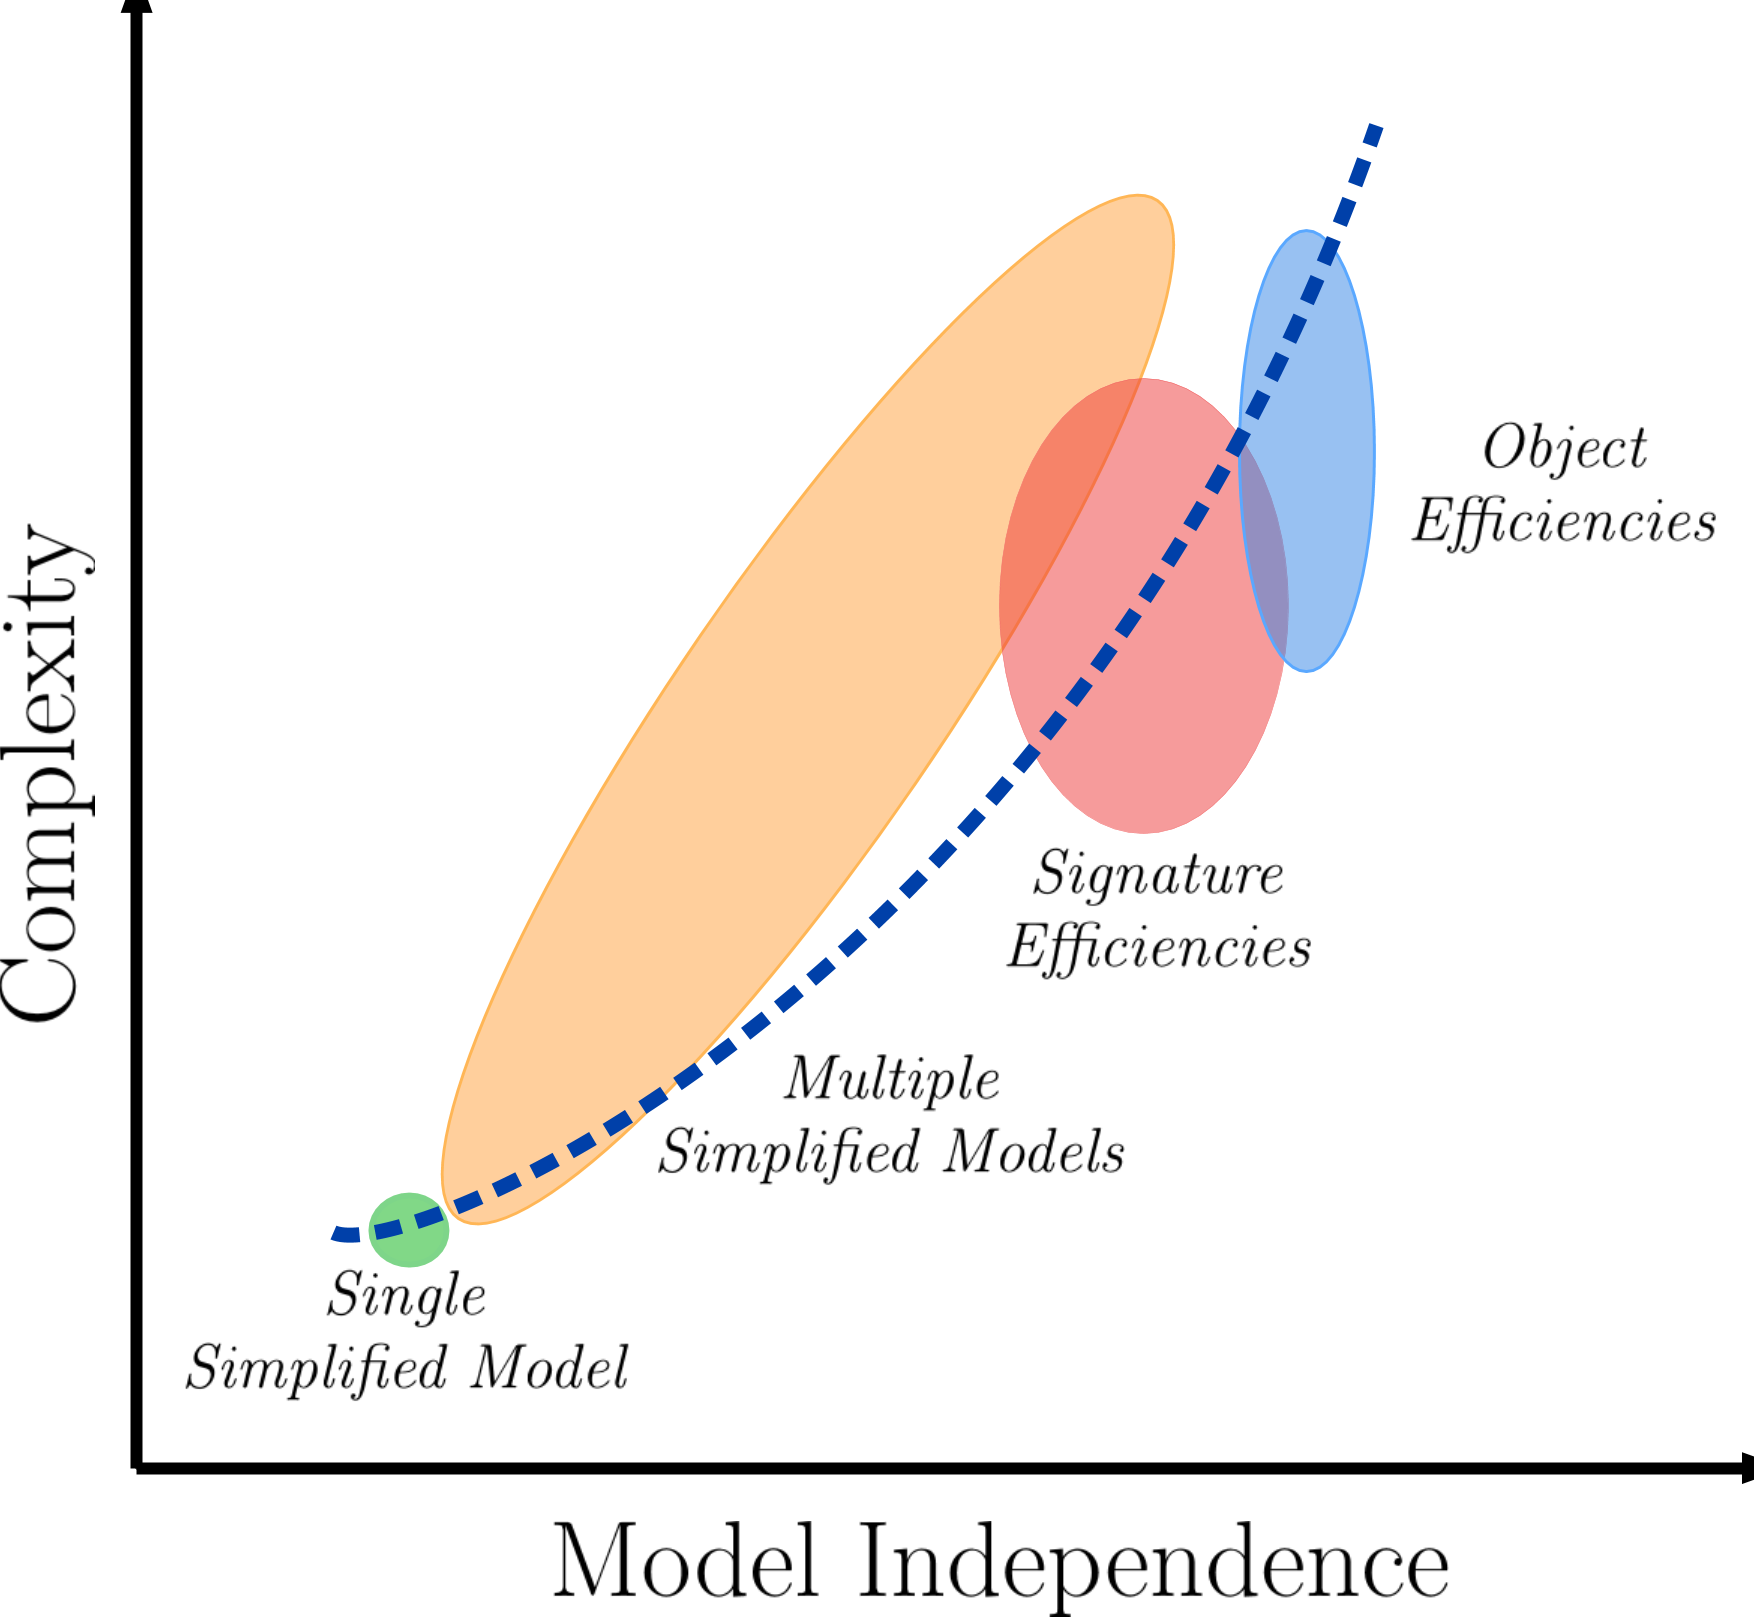
\includegraphics[width=0.7\textwidth,angle=0]{ch5-figures/LLP_interpretationsB.png}
\end{center}
\caption{A qualitative overview of the possibilities
for results presentation discussed in this chapter.
The axes represent the complexity of information required by each
format and the corresponding level of model independence.}
\label{fig:ch5-complexity-vs-modelindependence}
\end{figure}

The objective of this chapter is to discuss the presentation of the LLP search results  
with the aim that they can be re-used for interpretations beyond the models considered in the 
experimental publications.  
To this end, we first discuss in Section~\ref{sec:ch5-options} the various options 
for presenting the LLP results, see Fig.~\ref{fig:ch5-complexity-vs-modelindependence}, and compare their advantages and
shortcomings. 
In Section~\ref{sec:ch5-smsReinterpretations} we discuss in more details how the simplified models defined in Section~\ref{sec:simplifiedmodel} can be used to re-interpret LLP searches. 
In Section~\ref{sec:ch5-recastExamples}, we present several attempts of recasting LLP searches, 
according to the LLP signature: heavy stable charged particles,
disappearing tracks and displaced objects; for each case, the lessons learned are elaborated. 
Section~\ref{sec:ch5-recastingDelphes} presents a first attempt to
extend the public detector simulator \textsc{Delphes} %and the recasting tool MadAnalysis5 
to deal with LLP searches, while 
Section~\ref{sec:ch5-recastingInsideExp} deals with reinterpretations performed within the experiments themselves, 
including the RECAST framework.  
In Section~\ref{sec:ch5-recastingPrompt}, we discuss complementary constraints on LLPs from re-interpreting prompt searches. 
We conclude in Section~\ref{sec:ch5-rec_summary} with our %suggestions and 
recommendations for the presentation of LLP results. 


%%%%%%%%%%%%%%%%%%%%%%%%%%%%%%%%%%%%%%%%%%%%%%%%%%%%%%%%%%
\section{Options for Presenting Experimental Results} 
\label{sec:ch5-options}
%%%%%%%%%%%%%%%%%%%%%%%%%%%%%%%%%%%%%%%%%%%%%%%%%%%%%%%%%%

A qualitative view of the various possibilities for presentation
of search results is given in
Fig.~\ref{fig:ch5-complexity-vs-modelindependence}.
We broadly classify these possibilities according to the type of
information provided or type of efficiency.
Each type refers to distinct signal objects, as illustrated in
Fig.~\ref{fig:ch5_presentation_options}.
As we can see, each possibility relies on distinct assumptions about
the signal, resulting in different levels of model-dependence.
Below we provide a brief discussion of the advantages and limitations of the
various possibilities of presentation of LLP search results.
We will gradually progress from the simplest case towards more complexity but
also better re-usability.


% Let us start with the presentation of results in the context of simplified
% models (for a list of proposed simplified models see {\color{blue}{Chapter~\ref{whitepaper:simplified-models}}}).
{\bf Simplified Models}: %the most commonly used format for the presentation of
%results is simplified model upper limits or efficiencies.
In most cases the simplified-model topology corresponds to single or pair
production of the LLPs, though in principle simplified models for production
through cascade decay of heavier states can also be envisaged. 
In any case, the simplified model incorporates important assumptions 
on the LLP production, decay mode and quantum numbers. 
%The search results are typically presented as  95\% CL limit curves, cross section upper limits and/or signal efficiencies.
Simplified-model results can be presented at different levels of sophistication and re-usability:
\begin{itemize}
\item exclusion curves in, e.g., a mass-vs-mass or mass-vs-lifetime plane, are highly model dependent and can 
rarely be used for re-interpretation;
\item cross-section upper limits\footnote{For the sake of re-usability, cross section upper limits in absolute terms are much preferred over limits on the signal strength.} 
can be applied to a larger variety of models
in which the same LLP production and decay mode occurs 
through a rescaling of the cross section times branching 
ratio factor; 
\item simplified-model efficiencies allow to go one step further: they make
it possible to combine different topology contributions to the same signal
region and compute an approximate likelihood using the number of expected and
observed events.
\end{itemize} 

% \noindent
The main advantages of simplified models are a parametrization in terms of few
physical parameters and a unified language and format applicable to a wide range of searches.
Also, when re-using simplified-model results one avoids detector simulation uncertainties. 
The disadvantages are that the simplified-model result  
cannot be applied to other LLP production or decay modes, resulting
in too conservative limits if the LLP signal is composed from
multiple topologies. This can be considerably relevant if 
the LLP is a color singlet, but there are several heavier color-charged states
which can be produced and decay to the LLP.
In principle this can be overcome if efficiencies are provided for a
sufficiently large number of simplified models (including cascade decays), as a
function of the simplified-model parameters, which should include the LLP lifetime.
These efficiencies can then be combined in order to compute the corresponding
constraints to complex models, where multiple topologies are present.
\footnote{These points are illustrated by the re-interpretation of the CMS search
for heavy stable charged particles~\cite{Khachatryan:2015lla}
discussed in Section~\ref{sec:ch5-smsReinterpretations}: 
for the specific model considered in \cite{Heisig:2015yla},
constraints obtained using only a single simplified model (direct production of
$\tilde{\tau}$s in this case) can underestimate the bounds on the LLP mass by almost a factor of two.}
We stress, however, that in order for this combination to be possible, signal efficiencies and 
not cross-section upper limits must be provided.
The major drawback of this approach is that in order for the results to be
applicable to a broad class of models, the number of required simplified models
and their complexity can easily become very large.
For achieving a high level of model independence, it is therefore desirable 
that the experimental analysis can be recast with Monte Carlo event simulation. 
Two ways of presenting results are useful to this end: {\it signature
efficiencies} and {\it object efficiencies}. 



\begin{figure}[t]
\begin{center}
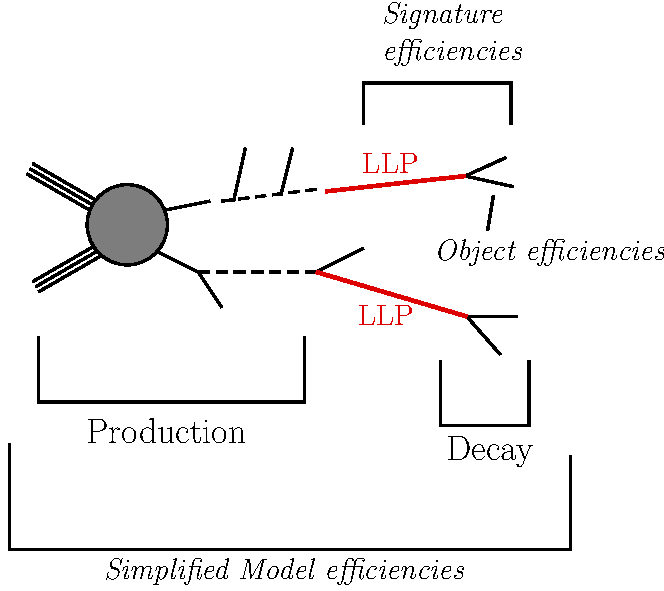
\includegraphics[width=0.6\textwidth,angle=0]{ch5-figures/LLPdiagramScheme.pdf}
\end{center}
\caption{Possibilities for the presentation of results: 
simplified-model efficiencies assuming a specific topology of LLP production and decay, 
signature efficiencies assuming only a specific LLP decay, and object efficiencies which are 
independent of the specific decay mode.
}
\label{fig:ch5_presentation_options}
\end{figure}


  
{\bf Signature efficiencies} are efficiencies for the reconstruction of the
main LLP signature (single charged track, displaced vertex, disappearing
track, \ldots) as a function of the LLP kinematical parameters and
the lifetime. 
Signal efficiencies require the assumption of a specific LLP decay, but 
are highly model independent, since they make no assumption on the LLP
production mode.
In addition, they are fully model-independent for stable particles
(within the detector dimensions), since in this case no assumptions about
the LLP decay mode are required.
In many cases, however, the reconstruction efficiencies depend on multiple
variables, such as the LLP $p_T$, its transverse decay position, impact
parameter, etc. 
As illustrated in section~\ref{sec:ch5-displacedVertices}, these efficiencies
could be very useful for recasting LLP searches, but often they 
are not provided by the experimental collaborations. Many recasting efforts consist in 
extracting these efficiencies from the provided information, but can result in large uncertainties. 

{\bf Object efficiencies} are efficiencies for the reconstruction of
the physics objects relevant for building the LLP signature. 
They can clearly be applied to a wide range of LLP
decay and production modes, since no specific assumptions about these are
required. 
For instance, a displaced lepton reconstruction efficiency can be provided
as a function of the lepton $p_T$ and its production position.
As discussed in Section~\ref{sec:ch5-displacedLeptons}, these efficiencies
can be used to recast LLP searches to an acceptable accurary ($\sim 20\%$).
Furthermore, as illustrated in Section~\ref{sec:ch5-displacedVertices},
knowledge of object efficiencies are essential for a general purpose
recasting of the search.
Within this approach the model dependence is minimal and can be
restricted to a few general assumptions about the nature of the LLP.
Also, object efficiencies could be included in fast
detector simulators, thus providing a way of recasting LLP searches
on the same footing as prompt searches. 
The main difficulty with providing such object efficiencies is
the potentially large number of parameters required for their parametrization.

